
\setcounter{section}{1}

\subsection{Indication sur les méthodes associées aux chaînes de caractères}

Les attributs suivants s'appliquent à des variables de type de chaîne de caractère :
\begin{itemize}
\item \pyv{.isalpha} renvoie \pyv{True} si c'est une des 26 lettres de l'alphabet et \pyv{False} sinon.
\begin{pyconsole}
'c'.isalpha()
'1'.isalpha()
\end{pyconsole}
\item \pyv{.index(x)} renvoie l'indice de la première occurrence de \pyv{x} :
\begin{pyconsole}
'hello'.index('l')
\end{pyconsole}
\item \pyv{.count(x)} renvoie le nombre d'occurrences de \pyv{x} :
\begin{pyconsole}
'hello'.count('l')
\end{pyconsole}
\end{itemize}

\subsection{Le chiffre de César}



Le \textbf{cryptage de César} est un des tout premier code de cryptage qui ait existé. 

La méthode est simple : il suffit de décaler toutes les lettres de l'alphabet du même nombre de lettres. 



Par exemple en choisissant un décalage de 3, le A devient le D, le B devient le E, le C devient le F et ainsi de suite. Pour la fin de l'alphabet, il suffit de revenir au début : le W devient Z, le X devient A, le Y devient B et le Z devient C. Ainsi un message comme "la metamorphose" devient par décalage d'une lettre "mb nfubnpsqiptf", ce qui est incompréhensible pour le non initié.


\question{Avec des instructions python, définir trois chaînes de caractères nommées \textit{alphabet}, \textit{mess} et \textit{code} contenant respectivement les caractères de l'alphabet, un message à crypter (exemple "la metamorphose") et le message crypté (vide initialement). On se limitera à des lettres minuscules non accentuées. Les autres caractères (espaces, chiffres...) seront gardés tels quels (non cryptés).}





\question{En utilisant les fonctionnalités découvertes dans la première partie, établir un algorithme permettant de crypter un message par le code de César, pour un décalage $n$ donné. Pour cela, mettre en place une boucle sur les caractères de la chaîne \textit{mess} et remplacer chaque lettre de \textit{mess} par la $n^{ieme}$ lettre suivante. Coder cet algorithme en Python et le tester sur le message "la metamorphose" avec une valeur de \textit{n=3}.}


\question{Proposer ensuite l'algorithme de décryptage qui affiche le message crypté en clair, en supposant que $n$ est inconnue. L'utilisateur choisira parmi les décryptages proposés celui qui a du sens ! Ecrire en langage python cet algorithme.}



\question{Pouvez-vous décrypter ce message secret intercepté dans un couloir du lycée : {\em "xq bdaotmuz pqhaud eqdm gz egvqf pq yapqxuemfuaz"}. Quelle est la faiblesse de ce type de code ?}



\subsection{Le chiffre de Vigenère}

\begin{figure}[!htb]
\begin{minipage}{0.5\textwidth}
On étudie maintenant la méthode de chiffrement de Vigenère. Pour comprendre le système de chiffrement, on commence par créer la table  Vigenère : on recopie $26$ fois l'alphabet en ligne, et à chaque saut de ligne on décale d'une lettre vers la droite comme sur la figure \ref{fig:vigenere}.

Cet algorithme fonctionne à l'aide d'une clé de chiffrement : une chaine de caractère (typiquement un mot).

Prenons un exemple, mettons que l'on veuille coder \og anticonstitutionnellement\fg~avec la clé \og roue\fg~. Pour ce faire, on crée le tableau présenté table \ref{TabVig} dont la première ligne contient le message à coder, et la deuxième la clé répétée autant de fois que nécessaire pour atteindre la longeur du texte à coder. On fait alors une lecture colonne par colonne de ce tableau et dans chaque colonne :
\begin{enumerate}
\item la première ligne donne l'abscisse dans la table de la lettre à coder;
\item la deuxième donne l'ordonnée dans la table de la lettre à coder;
\end{enumerate}
Ainsi le chiffrement du mot \og anticonstitutionnellement\fg~ avec la clé \og roue\fg~ est obtenue dans la table \ref{TabVig}.
\end{minipage}
\begin{minipage}{0.5\textwidth}
	\centering
		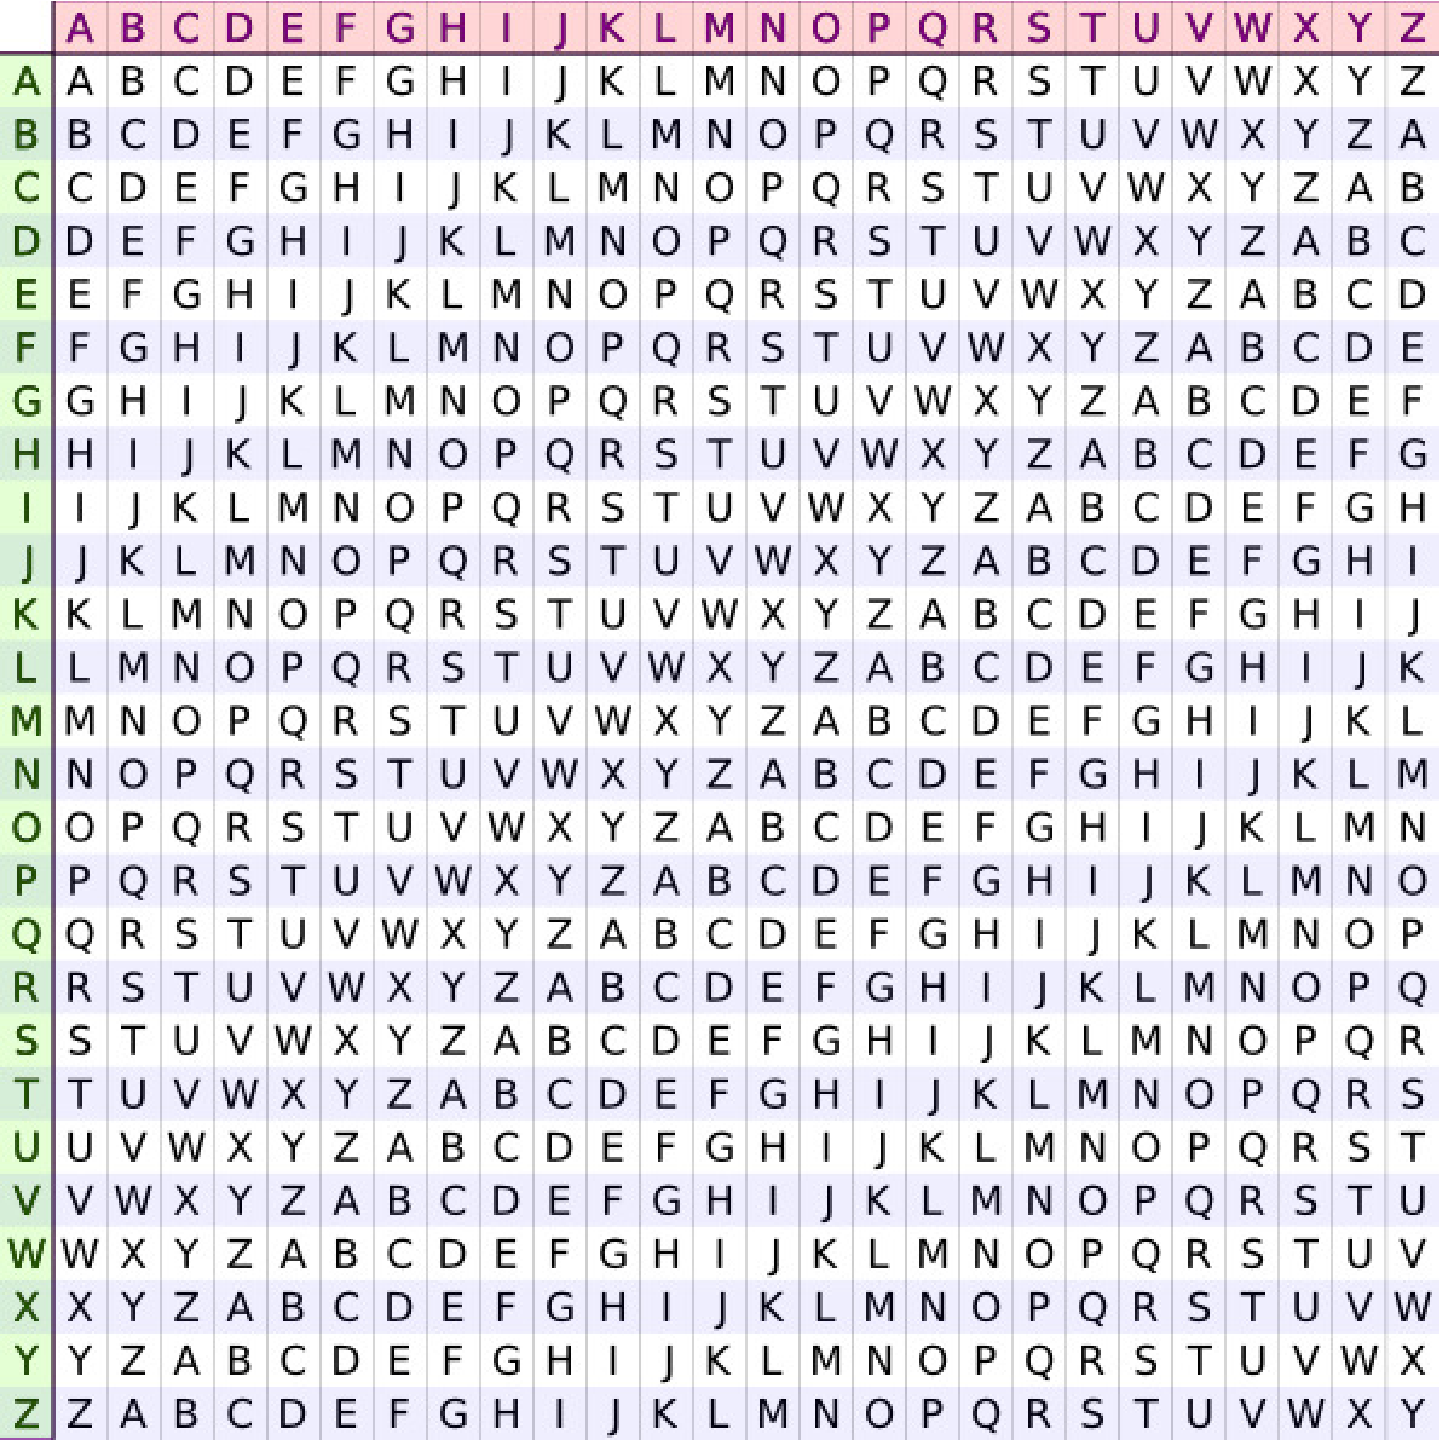
\includegraphics[width=0.95\textwidth]{vigenere.pdf}
	\caption{Table de Vigenère}
	\label{fig:vigenere}
\end{minipage}
\end{figure}




\begin{table}[htbp]
	\centering
		\begin{tabular}{l|*{25}{|c}}
			mot & a & n & t & i & c & o & n & s & t & i & t & u & t & i & o & n & n & e & l & l & e & m & e & n & t \\
			\hline
			clé & r & o & u & e & r & o & u & e & r & o & u & e & r & o & u & e & r & o & u & e & r & o & u & e & r \\
			\hline
			code & r & b & n & m & t & c & h & w & k & w & n & y & k & w & i & r & e & s & f & p & v & a & y & r & k \\
			\hline
		\end{tabular}
		\caption{Exemple de chiffrement de Vigenère}
		\label{TabVig}
\end{table}


La méthode de chiffrement par lecture de la table est une méthode adaptée \og aux humains\fg, ainsi on réfléchira à l'implémentation d'un algorithme plus efficace en s'aidant de l'exemple.

\question{Écrire une fonction \texttt{code\_vigenere(ch,cle)} ayant pour paramètre d'entrée une chaîne de caractères \texttt{ch}, la clé \texttt{ch} et pour résultat la chaîne \texttt{ch} codée : \texttt{chcode}.}

\question{Écrire une fonction \texttt{decode\_vigenere(chcode,cle)} ayant pour paramètre d'entrée une chaîne de caractères \texttt{chcode}, la clé \texttt{ch} et pour résultat la chaîne \texttt{chcode} décodée : \texttt{chdecode}.}

\question{Quel est selon vous l'intérêt de ce codage par rapport à l'algorithme de César ?}

\vspace{0.5cm}

